\chapter{Implementation}
This chapter discusses the implementation details of the proposed mobile application. First, the \gls{har} stages will be discussed. That includes the data gathering process from the project participants as well as data prepossessing and training of the kNN classifier. Next, the self-management system will be discussed followed by the specifics of the mobile application itself such as database and overall system design implementation.

\section{HAR System}
In order for the system to take actions such as notifying the user for a prolonged periods of inactivity or sending a notification when a \gls{pa} goal is achieved, the application needs to recognise human activities (i.e. walking and running). Implementation of the \gls{har} system will be discussed bellow.

    \subsection{Data Collection}
    One of the key stages in the development process of a typical supervised (online) \gls{har} system is the data collection stage. A labelled dataset is needed in order to train a model (or also called classifier). The produced model can classify an "unseen" (or unlabelled) data to a specific activity (i.e. walking or being static).
    
    \subsubsection{Setting and project participants}
    The data needed to train the model in this work was collected from 3 fellow students in a controlled environment. Each one of the project participants was equipped with a device running partially implemented \textit{"Active Minutes"} application (e.g. only the \textit{"Data Collection screen"} see \ref{fig:data-collection-screen-design}). Before performing the data collection process, the participants had to, first, select the activity they will perform from a list of activities and then press the Start button on the application's UI in order to start the data collection process. The location of the device during the recording was chosen to be the front pants pocket. This location has been found to be the optimal position for \gls{har} (see \ref{section:non-commercial-har-systems}). All of the participants recorded 3 minutes of each one of the following activities: \textit{walking}, \textit{running}, \textit{cycling} and \textit{static}. To avoid any unwanted information during the recording stage, the first and the last 7 seconds of each activity was removed since it contained noise information such as the linear acceleration taking place when the device was put in and pulled out of participants pockets. That was pragmatically done and no direct human intervention was needed to further filter the data.
    
    \subsubsection{Recorded data}
    \label{subsubsection:recorded_data}
    When all of the required data was collected, it was converted into a WEKA ARFF file format by pressing the "EXPORT" button on the Data Collection screen. The ARFF file was stored on the device's external memory (e.g. SD card). A sample of the produced ARFF file can be seen in Appendix \ref{chapter:arff-dataset-sample}. A dataset containing ~720 labelled data points (or a total of ~36 minutes of data) was produced as a result of the data collection process. 
    
    The device used to collect the data was \textit{OnePlus One} equipped with low-power high performance 3-axes accelerometer \footnote{\url{http://www.st.com/en/mems-and-sensors/lis3dh.html}}. As for the sampling frequency (SF) of the sensor, the Android Operating system provides a total of four different sampling frequencies for reading the accelerometer sensor, namely \textit{NORMAL: 5 Hz}, \textit{UI: 16 Hz}, \textit{GAME: 50 Hz}, and \textit{FASTEST}. The latter has been chosen for the SF of the built-in accelerometer as it has produced good results in \citet[3-5]{lee2016}. According to the Google's documentation \textit{FASTEST} SF depends on the hardware of the device \citep{googlesensormanager2017}. In this case, the SF was \textbf{115} Hz. 
    
    \subsection{Training the kNN classifier}
    The exported ARFF Weka file (see section \ref{subsubsection:recorded_data}) is then bundled into the application itself by transferring the collected data straight into the \textit{Assets} directory of the mobile application. That allows for "shipping" the application with the collected training dataset. The \gls{knn} classifier is then trained and serialised when the \textit{onCreate} method of the \textit{Application} is called. This method is only called once during the life of the application \citep{googleapplication2017}.
    
    \subsubsection*{Accuracy}
    The ARFF Weka file (dataset) was tested externally on a PC to find the optimal \gls{knn} parameters such as the number of neighbours the classifier should consider before making a class prediction as well as whether to perform a cross validation of the data. The testing was done using the PC version of WEKA \footnote{\url{http://www.cs.waikato.ac.nz/ml/weka/}} Machine Learning application. After performing thorough testing, the default parameters of the \gls{knn} classifier performed the the best reaching accuracy of \textit{83.7\%} for dataset containing 763 data points. The performance for the trained model can be seen in table \ref{table:4_class_confusion_matrix}. 

    \begin{table}[ht]
    \centering
    \begin{tabular}{ |c|c|c|c||c| } 
     \hline
     a & b & c & d & classified as\\
     \hline \hline
     140 & 4 & 2 & 33 & a = walking \\
     57 & 112& 0 & 10 & b = running \\
     0 & 1 & 218 & 0 & c = static \\
     5 & 1 & 11 & 169 & d = cycling \\
     \hline
    \end{tabular}
    \caption{4 classes Confusion Matrix}
    \label{table:4_class_confusion_matrix}
    \end{table}

According to the confusion matrix in the table above, data points of class "running" has been incorrectly classified 57 times as class "walking" and 10 times as class "cycling". However, for the implementation purposes of the proposed application that performance of the model is still acceptable because even though the classifier has been designed to distinguish between 4 classes, only 2 classes are taken into account, namely "static" and "active" (including "walking", "running" and "cycling") on a programming level. Feature versions of the application may utilise the "active" classes to show a more detailed information to the user such as how much time the user has spend walking or running throughout the day.

To demonstrate the actual accuracy of the model taking account only those 2 classes, the original dataset has been modified so that only 2 classes are present - static and active. The confusion matrix after training the model(again the same \gls{knn} classifier with default parameters) can be seen in table \ref{table:2_class_confusion_matrix}. The actual accuracy of the classifier reaches 98.1\% since only 14 data points has been incorrectly classified.

    \begin{table}[ht]
    \centering
    \begin{tabular}{ |c|c|c| } 
     \hline
     a & b & classified as\\
     \hline \hline
      531 & 13 & a = active\\
      1 & 218 & b = static\\
     \hline
    \end{tabular}
    \caption{2 classes Confusion Matrix}
    \label{table:2_class_confusion_matrix}
    \end{table}
    
    \subsection{HAR System Implementation}
    The basic architecture of the \gls{har} system integrated into the application has been informed by \citet[149]{labrador2013}. For example, classes such as \textit{Point}, \textit{TimeSeries}, \textit{TimeWindow}, \textit{FeatureSet} and \textit{FeatureExtractor} form the core of the \gls{har} system. Simplified diagram of the \gls{har} system can be seen in figure \ref{fig:har_system_impl_class_diagram}. The HAR system is integrated in the \textit{ActiveMinutesService} mentioned in section \ref{section:architectural-design} so it can recognise and provide the recognised activities to \textit{ActivityMonitor} class which will be discussed shortly. A brief discussion on the main responsibilities of the HAR system classes is presented bellow.
    
    \begin{figure}[ht]
        \centering
        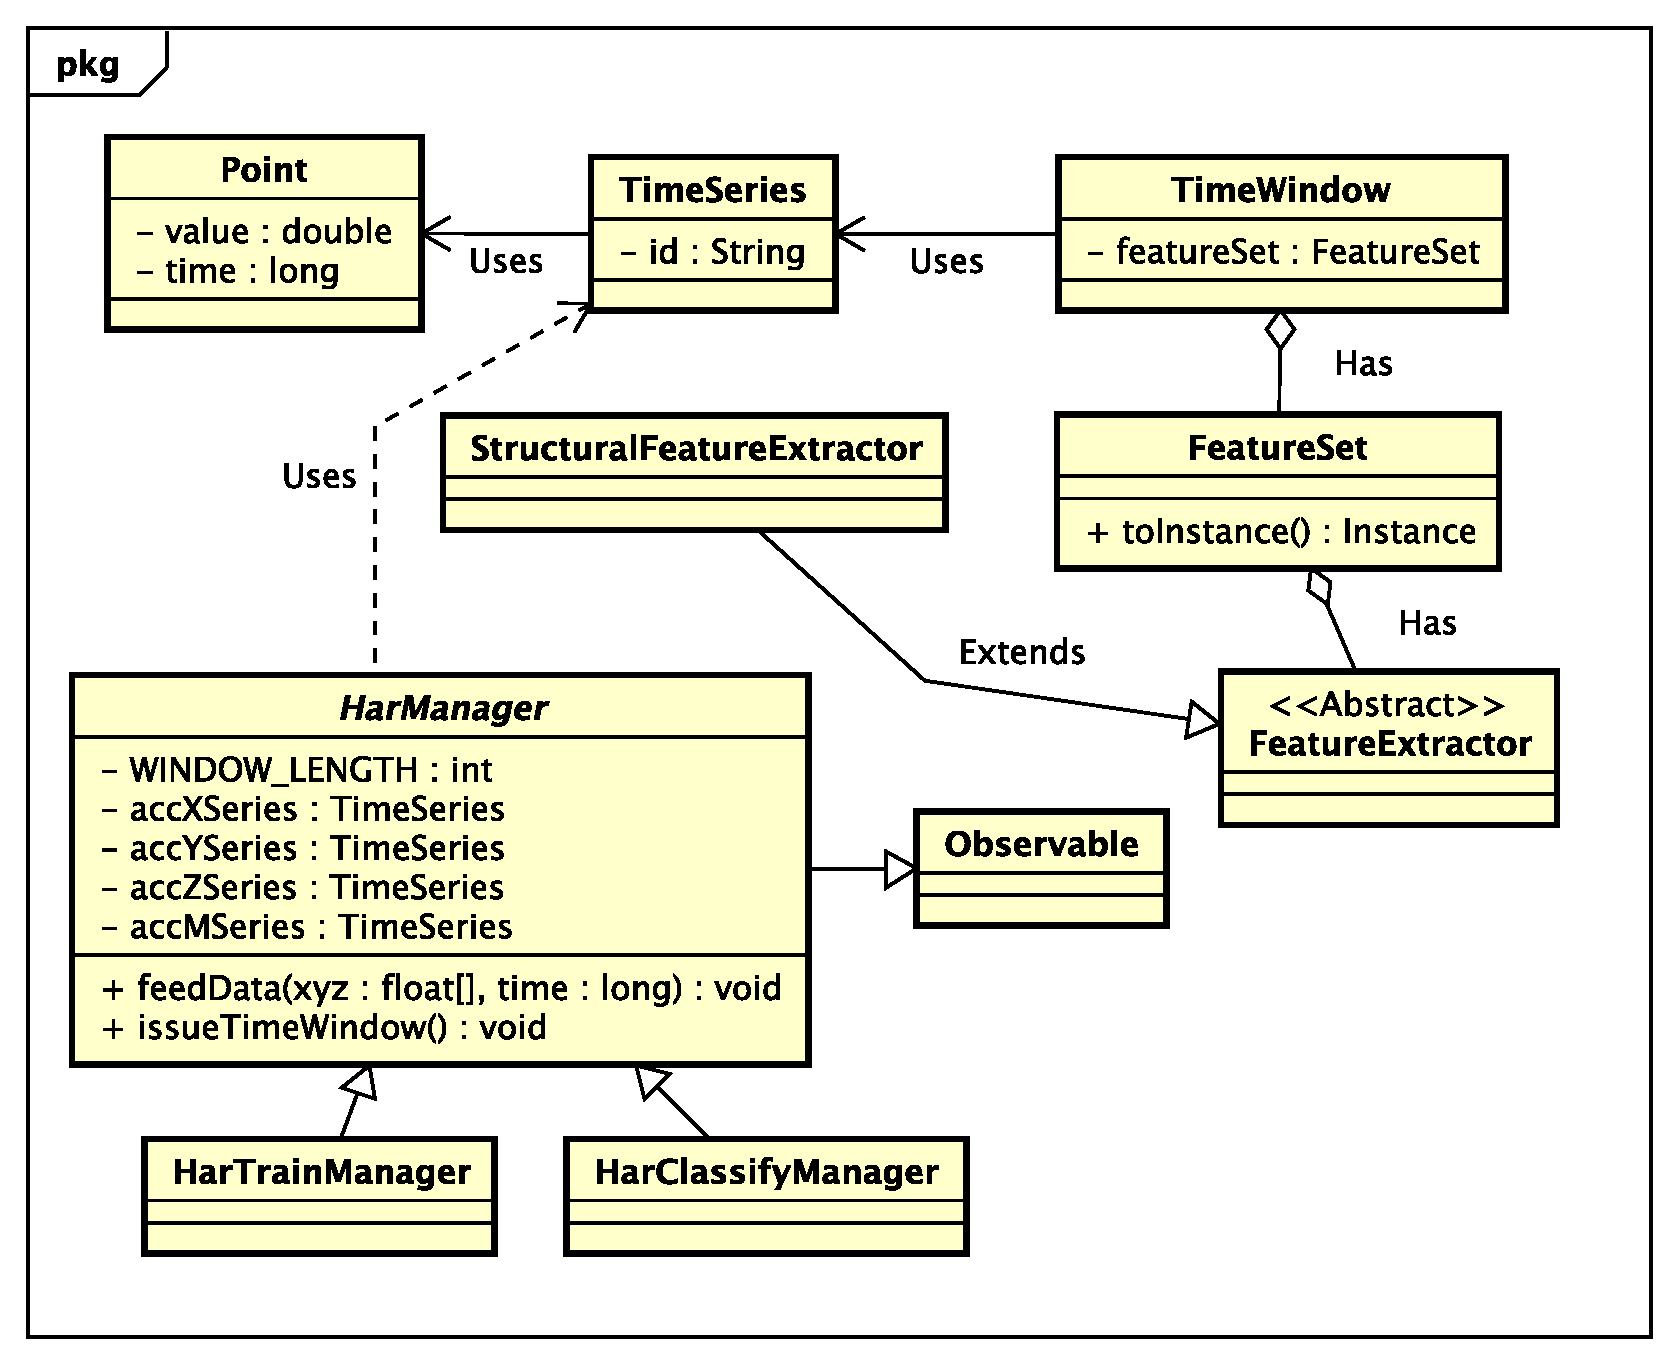
\includegraphics[width=13cm]{har_system_class_diagram_pdf}
        \caption{HAR system class diagram (simplified)}
        \label{fig:har_system_impl_class_diagram}
    \end{figure}
    
    Class \textbf{Point} is responsible for storing the readings of the smartphone accelerometer sensor. Every instance of the class stores the accelerometer readings such as the amount of acceleration in X, Y and Z direction in a class variable \textit{value} as well as a \textit{time} class variable which is used to compare different instances of the class.
        
    \textbf{TimeSeries} class extends \textit{ArrayList} which is one of the widely used data structure in the Java language since it allows easy storing and manipulation of list of items \citep{oraclearrayList_2017}. TimeSeries class stores a list of \textit{Point} values labeled by an \textit{id} value (see figure \ref{fig:har_system_impl_class_diagram}). For example, to store the accelerometer \textit{X} direction acceleration values in a TimeSeries instance, its \textit{id} could store value such as "accX".
        
    \textbf{TimeWindow} class extends Hashtable. That allows for storing values accessed by key \citep{oraclehashtable_2017}. For example, TimeWindow class provides means of storing \textit{TimeSeries} objects and accessing them via key. The key value used to associate every TimeSeries object is the same as the \textit{id} value of the TimeSeries object itself.
    
    \textbf{StructuralFeatureExtractor} is a class that extends the abstract class FeatureExtractor. The reason behind this abstraction is that in the future more extractors can be added such as \textit{StatisticalFeatureExtractor} which could extract statistical data features from a dataset such as mean or standard deviation. StructuralFeatureExtractor is responsible for extracting the structural data features such as the first 5 coeficients of the \gls{fft} algorithm for all of the accelerometer axis and their magnitude as described in section \ref{section:proposed-application}.
    
    \textbf{FeatureSet} class is responsible for storing the extracted data features of the \textit{StructuralFeatureExtractor}. Similarly to TimeWindow, this class extends Hashtable as well. The key in this case is a combination between the id of the TimeSeries instance and the name of the feature such as "\_fft". The value that can be accessed by this key is the value of the specific TimeSeries \gls{fft} coefficient. For example, if we want to store the FeatureSet (e.g. feature vector) of \textit{TimeSeries} with id = "AccX" (e.g. the values of the accelerometer in X direction for a given time) the key to access the first \gls{fft} coefficient of this TimeSeries would like that \textit{"AccX\_fft1"}.
    
    \textbf{HarManager} is a class that manages the raw data from the smart phone's accelerometer. The data is delivered in the class via its method \textit{feedData}. This method accepts an array of float values \textit{xyz} which are the readings of the accelerometer at a given time. The method feeds data into the appropriate TimeSeries (i.e. accXSeries). When the window length is reached (e.g. 3 seconds) the method \textit{issueTimeWindow} is called. The purpose of this method is to extract data features from the raw data. The two direct subclasses of HarManager class - \textit{HarTrainManager} and \textit{HarClassifyManager} override the method so that it stores the labelled data points during the data collection process or classifies the unseen (or unlabelled) data points during the classification or monitoring process. For example, the \textit{DataCollectionService} class discussed in section \ref{section:architectural-design} uses an instance of the HarTrainManager class to collect data and train \gls{knn} classifier. On the other hand, the HarClassifyManager is used in the main service of the application called "ActiveMinutesService" (again discussed in section \ref{section:architectural-design} to classify unseen instances periodically). 
        
        
\section{Self-Management System}
This section discusses the implementation of self-management system. Its responsibilities include monitoring the user's activity levels as well as providing feedback upon reaching a specific threshold. A class diagram of the system can be seen in figure \ref{fig:self_management_system}. The following subsections will discuss the main components of the self-management system. 

\begin{figure}[ht]
    \centering
    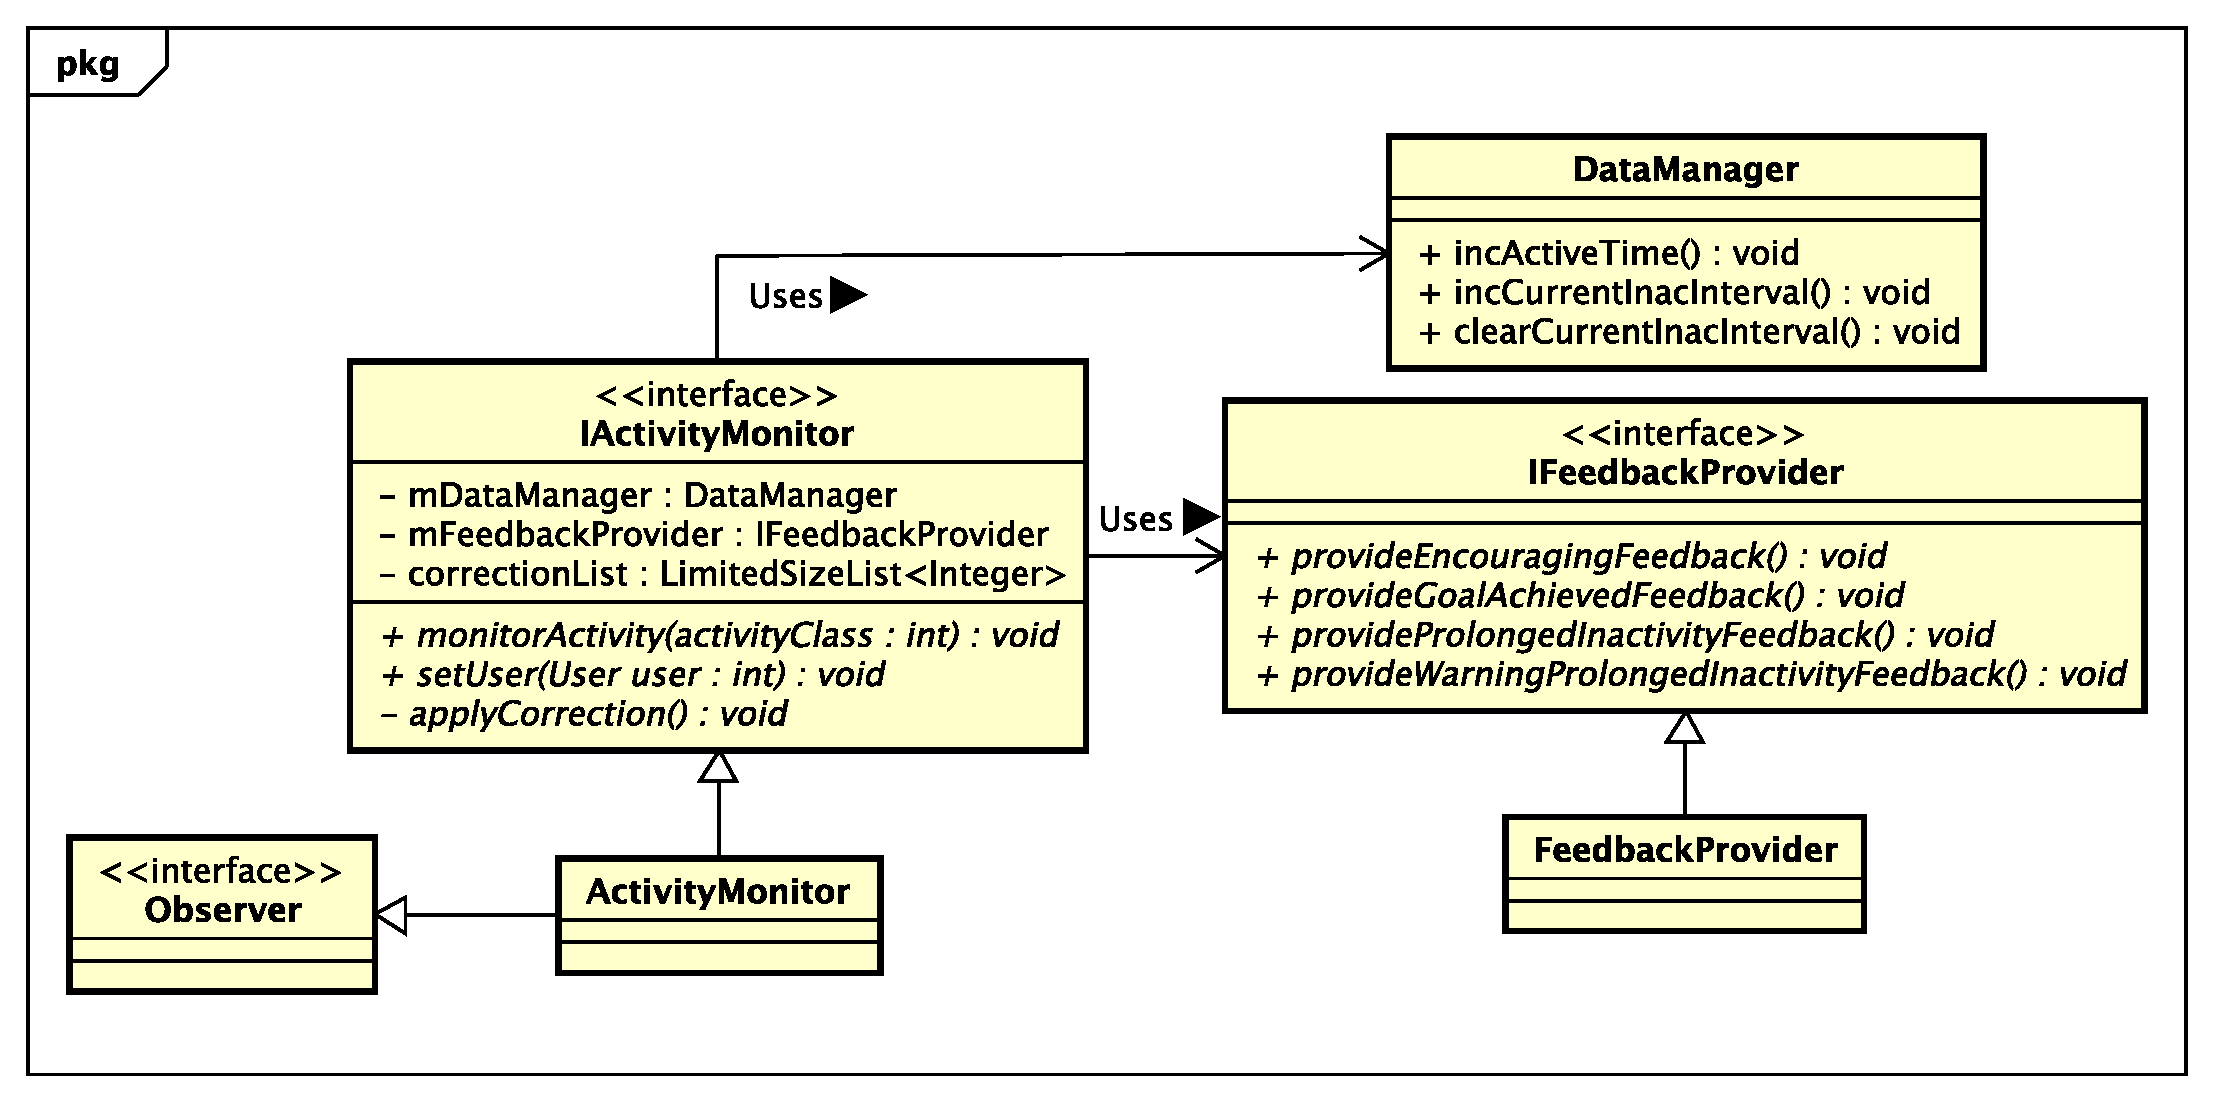
\includegraphics[width=12cm]{self-management-system-class-diagram}
    \caption{Self-Management System class diagram (simplified)}
    \label{fig:self_management_system}
\end{figure}

    \subsubsection{ActivityMonitor}
    As the name implies, this class monitors user's \gls{pa} and \gls{st} levels. ActivityMonitor accesses the previously set daily physical activity and maximum continuous inactivity goals set by the user. The User object that this class needs is provided by a method called \textit{setUser(User user)}. The details of how the user is set will be discussed in more detail in a subsequent section.
    
    One of the most important methods of the class is called \textbf{monitorActivity(activityClass: int)}. This method is called by the \textbf{HarManager} mentioned above as soon as an activity type is recognised (every 3 seconds). It passes the recognised activity to the ActivityMonitor via the method mentioned above. ActivityMonitor then is able to react on the activity type. For example, if the activity type is of type \textit{Static}, ActivityMonitor calls the DataManager's \textit{incCurrentInacInterval()} method which increments the current inactivity interval in the database.
    
    \subsubsection{Frequent positions changes}
    One problem that had to be solved during the implementation of this class was dealing with the frequent changes of the device position. For example if the user pulls out their phone (e.g. to check for missed calls) and put it back in the pocket, these series of events are usually interpreted by the HarManager as activity class of type Active (e.g. running, walking or cycling). Without applying any kind of data filtering ActivityMonitor will increment the user's active time incorrectly especially if the user is static at the time of the interaction with their phone. Consequently, that will lead to wrong activity data and potentially misleading the user.
    
    After series of experiments it was found that by storing the last 3 recognised activities in a list (i.e. walking, running, walking) and comparing them with the "current" activity, these frequent device changes are dramatically avoided. That is because, in order for the activity to be classified as \textit{Active} all of the activities in the list must be of the same \textit{Active} type (i.e. walking, running or cycling). Pragmatically, this is achieved by a method called \textit{applyCorrection()}. The interested reader can find the implementation of \textbf{ActivityMonitor} class in Appendix \ref{chapter:activity-monitor-class}.
    
    \subsubsection{DataManager}
    As can be seen in figure \ref{fig:self_management_system} a reference of this class is used in \textit{ActivityMonitor}. The role of \textbf{DataManager} is to provide methods of manipulating the underlining database so that it is relevant to the needs of \textit{ActivityMonitor}. For example, \textit{ActivityMonitor} receives a recofnised activity of type \textit{Active} (i.e. walking), \textit{ActivityMonitor} calls \textit{incActiveTime()} and \textit{clearCurrentInacInterval()} consequently. The former method increments the user's active time and the latter clears the current inactivity interval to 0.
    
    \subsubsection{FeedbackProvider}
    This class is responsible for providing information to the user in the form of Android notifications\footnote{\url{https://developer.android.com/reference/android/app/Notification.html}}. For example, when \textit{ActivityMonitor} detects that the user has reached their daily maximum continious interval (set sedentary goal) it would call \textit{provideProlongedInactivityFeedback()} method of the \textit{FeedbackProvider}.
    
    Notifying the user of past events specially associated with user's inactivity is not very helpful from a self-management perspective. Thus, the class has been designed to include two methods that are called at 80\% achieved goal progress, namely \textit{provideEncouragingFeedback()} and \textit{provideWarningProlongedInactivityFeedback()}. For example, if the \gls{st} goal i.e., maximum continious inactivity (MCI) is set to be 60 minutes per day. The user will receive a notification at 48 minutes of continious inactivity giving the user a warning that they are approaching their \gls{mci}. 

\section{"Active Minutes" application} 
This section will discuss the main and most interesting building blocks of the proposed software. First, the realisation of the database design will be addressed. Next, the \textit{ActiveMinutes Service} functionality will be discussed followed by the Application UI.  
    
    \subsection{Realm Database}
    As it was mentioned in section \ref{section:data-manager}, a library called \citet{realmdatabase_2017} is utilised to perform all the data management responsibilities. This third-party software was carefully chosen based on several factors. It offers Fast queries and Safe threading (accessing the data from many threads without conflicts). What is more, it saves a lot of time compared to implementing a database from scratch. The following sections will address how the database was implemented using the above-mentioned library. 
    %\subsection{Data collection service} Not sure if to include it
    
    \subsection{ActiveMinutes Service}
    
    \subsection{Application UI}  




    
    
    
    